\section{Proving your location}
As an increasing amount of personal information is accessible on the internet and therefore on mobile devices, we are losing the security that previously existed by requiring physical interaction between humans to transfer sensitive data

Location proof is a large part of that security. There is currently no ubiquitous method of \textit{proving} your location at a given time digitally. Many companies, such as Netflix, use GeoIP databases such as MaxMind \cite{maxmind} to estimate a users location based on his IP address. This technique is inaccurate and easily bypassable using proxy servers or VPNs.

One newer, more advanced tecnique of location observation is Constraint-Based Geolocation \cite{constraint-based}. This is an active geolocation technique, compared with GeoIP verification which is static. It estimates the location of a users IP address by calculating the latencies between the user's machine and multiple surrounding machines with fixed, known locations. However, even advanced systems like these can easily be bypassed, using IP spoofing techniques, proxy servers, VPNs, or by using anonymising networks such as TOR \cite{tor}.

Better solutions to this problem exist. \textit{Location proof systems} allow users of the system to \textit{prove} their location to another user, by creating \textit{location proofs}. Location proofs vary from system to system. In essence, a location proof is a piece of data, potentially signed or encrypted by another party, which attests the location of a user at a specific time. Examples of location proof systems are discussed in detail in section \ref{ssec:proof_systems}.

\section{Distributed and decentralised systems}
A \textit{distributed} system is a system which distributes the computation of a task across multiple nodes (computers) connected over a network. These nodes then work together and communicate to complete the task by passing messages over the network \cite{distributed}.

For example, Google search indexes are not computed on just one node, rather on a network of nodes that communicate by sending messages to each other. Google therefore \textit{distributes} the task of calculating search indexes across multiple nodes. This two main advantages; It is less time consuming, because different index calculations can be computed on different nodes at the same time, and it's scalable, because nodes can be added or removed from the network dynamically, to meet demand.

A \textit{decentralised} system is similar to a distributed system, except no node is in charge. Nodes in a decentralised network still communicate by passing messages to each other over the network, but unlike a distributed system, they arent assigned tasks by a central or master node. Bitcoin \cite{bitcoin} is a good example of a large-scale decentralised system. Two nodes in the Bitcoin network can choose to send money between themselves, creating a transaction. They make the details of that transaction public. The two nodes therefore create and publish the transaction iwithout coordination from a central node.

In the context of a location proof system, I consider a distributed location proof system to be one where the task of facilitating user proof request and creation is distributed across multiple \textit{worker nodes}, which are controlled and coordinated by a central node. This allows a higher volume of proofs to be created concurrently compared with using a single node, while maintaining centralised and simple control over the system. This is shown in figure \ref{fig:distributed_location}.

\begin{figure}[H]
\begin{center}
\resizebox {0.6\columnwidth} {!} {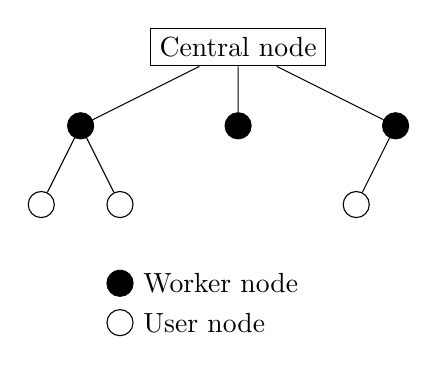
\begin{tikzpicture}

\node[draw] (C) at (0,0) {Central node};

\node[draw,style=circle,fill=black] (D1) at (-2,-1) {};
\node[draw,style=circle,fill=black] (D2) at (0,-1) {};
\node[draw,style=circle,fill=black] (D3) at (2,-1) {};

\draw[-] (C) -- (D1) (C) -- (D2) (C) -- (D3);

\node[draw,style=circle] (N1) at (-2.5,-2) {};\node[draw,style=circle] (N2) at (-1.5,-2) {};
\node[draw,style=circle] (N3) at (1.5,-2) {};

\draw[-] (N1) -- (D1) (N2) -- (D1) (N3) -- (D3);

\node[draw,style=circle,fill=black,label=right:Worker node] (L1) at (-1.5,-3) {};
\node[draw,style=circle,label=right:User node] (L2) at (-1.5,-3.5) {};

\end{tikzpicture}}
\end{center}
\caption{Distributed location proof system}
\label{fig:distributed_location}
\end{figure}

I consider a decentralised location proof system to be one where no node is in charge of controlling or coordinating the system. Nodes can create and publish location proofs between themselves, without the need for a central third party to coordinate the interaction (figure \ref{fig:decentralised_location}). This makes coordination more complex, but means that no node is considered to be ``in charge'' of the system.

\begin{figure}[H]
\begin{center}
\resizebox {0.6\columnwidth} {!} {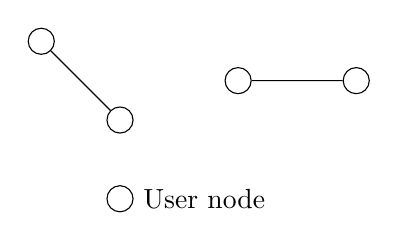
\begin{tikzpicture}

\node[draw,style=circle] (N1) at (-2.5,-1) {};\node[draw,style=circle] (N2) at (-1.5,-2) {};

\node[draw,style=circle] (N3) at (0,-1.5) {};
\node[draw,style=circle] (N4) at (1.5,-1.5) {};

\draw[-] (N1) -- (N2) (N3) -- (N4);

\node[draw,style=circle,label=right:User node] (L1) at (-1.5,-3) {};

\end{tikzpicture}}
\end{center}
\caption{Decentralised location proof system}
\label{fig:decentralised_location}
\end{figure}

\section{Existing location proof systems} \label{ssec:proof_systems}
Location proof systems are expected to be accurate and tamper-proof. For this reason, existing solutions \cite{brassil, luo, khan} have chosen to use a central authority to issue proofs, or to regulate proof issuance.

A hardware technique \cite{brassil}, developed by Brassil et al. of HP Laboratories, operates by supplementing existing WiFi access points (\textit{AP's}) with \textit{femtocells}. A femtocell \cite{femtocell} is a small cellular antenna that connects to a mobile carrier via the Internet, which allows mobile networks (e.g. networks used for calls and texts) to be extended on demand. Location verification over the internet is made possible by determining which femtocell a mobile node is connected to as it transfers data via Wi-Fi. This is possible because the central server in the location verification system has access to the mobile operator's user data.

This solution requires investment in additional hardware to supplement existing WiFi access points, and requires access to mobile providers' user database to identify users locations (see figure \ref{fig:hp_labs}).

\begin{figure}[H]
\begin{center}
\resizebox {0.5\columnwidth} {!} {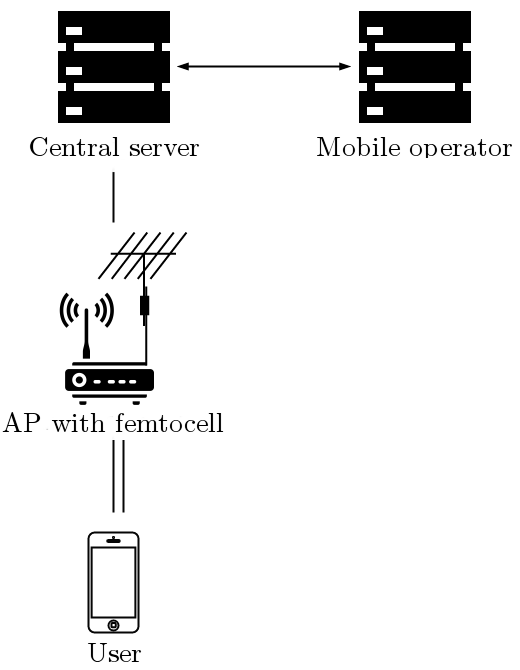
\includegraphics{diagrams/hp_paper.png}}
\caption{Hardware-based proof system (Adapted from Brassil et al. \cite{brassil})}
\label{fig:hp_labs}
\end{center}
\end{figure}

The use of a centralised system, as described above, creates security, privacy and vulnerability issues. An attacker who succeeds in compromising the security of the central server can violate the privacy of the users of the system, and potentially track their location. This is because in this system, location proof data resides with the central server. This means that the user has no control over the security of their proofs, and an attacker could sieze them. The central system architecture is also vulnerable, in the sense that a resource availability attack such as a DDoS attack \cite{ddos} could render the central architecture unavailable, making location verification unavailable.
\\

Luo et al. propose a system that uses software installed on Wi-Fi access points to allow users to create location proofs \cite{luo}. In their system, each access point is given a \textit{group signature} by a central server, and can sign location proofs for users (figure \ref{fig:luo_diagram}).

\begin{figure}[H]
\begin{center}
\resizebox {0.5\columnwidth} {!} {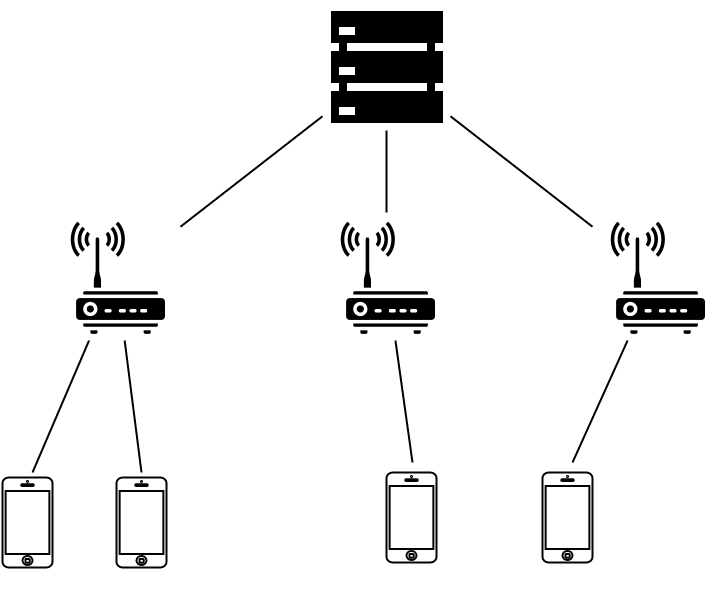
\includegraphics{diagrams/ap_paper.png}}
\caption{Access point proof system (Adapted from Luo et al. \cite{luo})}
\label{fig:luo_diagram}
\end{center}
\end{figure}

Users can request a location proof from any access point, and receive a proof encrypted by the AP with the group signature, as shown in figure \ref{fig:luo_transaction}. This can then be submitted to a Verifier.

\begin{figure}[H]
\resizebox {\columnwidth} {!} {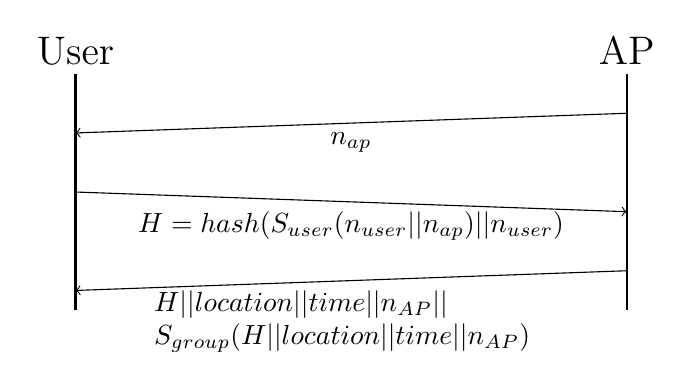
\begin{tikzpicture}
\coordinate (A_T) at (0,3);
\coordinate (A_B) at (0,0);
\coordinate (A_1) at (0,2.25);
\coordinate (A_2) at (0,1.5);
\coordinate (A_3) at (0,0.25);

\coordinate (B_T) at (7,3);
\coordinate (B_B) at (7,0);
\coordinate (B_1) at (7,2.5);
\coordinate (B_2) at (7,1.25);
\coordinate (B_3) at (7,0.5);

\draw[thick] (A_T)--(A_B);
\draw[thick] (B_T)--(B_B);
\draw (A_T) node[above]{\Large User};
\draw (B_T) node[above]{\Large AP};

\draw[->] (B_1) -- (A_1) node[midway,below] {$n_{ap}$};
\draw[->] (A_2) -- (B_2) node[midway,below]
	{$H = hash(S_{user}(n_{user} || n_{ap}) || n_{user})$};
	
\draw[->] (B_3) -- (A_3) node[text width=5cm,midway,below]
	{$H || location || time || n_{AP} ||$\\
	$S_{group}(H || location || time || n_{AP})$};
\end{tikzpicture}}
\caption{Proof encrypted with group signature (Adapted from Luo et al. \cite{luo})}
\label{fig:luo_transaction}
\end{figure}

This system creates \textit{proactive} location proofs. A proactive location proof is one which is created before it is needed. The user creates application-independent location proofs, and can use them at a later time with any application(s) he chooses.
\\

A system proposed by Khan et al. takes a different approach, by using other users as witnesses to a location claim \cite{khan}. In this system, a \textit{witness} physically located near the user is used by the central server to verify the user's location claim (figure \ref{fig:witness_paper}). Like the model proposed by Luo et al., this system allows the user to have control over their own privacy, as the user owns the location proof.

\begin{figure}[H]
\begin{center}
\resizebox {0.4\columnwidth} {!} {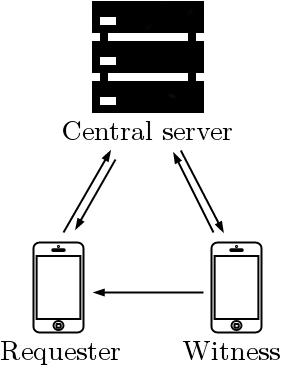
\includegraphics{diagrams/witness_paper.png}}
\caption{Proof system using witnesses (Adapted from Khan et al. \cite{khan})}
\label{fig:witness_paper}
\end{center}
\end{figure}

\section{Blockchain}
In Bitcoin \cite{bitcoin}, the entire transaction history is stored in the \textit{blockchain}. This is a decentralised, append-only ledger (database) \cite{blueprint}. The blockchain is maintained by a network of \textit{miner} nodes competing to collect transactions into a new block, sign that block by solving a difficult puzzle known as a \textit{proof-of-work}, and append it to the ledger. It is used in Bitcoin to enforce consensus; every miner in the network agrees that all blocks in the blockchain are valid, due to the presence of their associated proof-of-work.

A proof-of-work is a solution (a numerical value) to a problem which is computationally expensive to solve, but computationally cheap to verify that the solution is correct. As blocks are added to the blockchain, the amount of work required to generate the proofs-of-work for the entire chain increases. Because proof-of-work solutions also incorporate some information about the previous block in the chain, changing data inside a block in the blockchain would not just require regeneration of the proof-of-work for that block, but for all successive blocks as well. Therefore the blockchain is tamper-proof, assuming that the majority of the CPU power in the miner network is controlled by  honest nodes \cite{bitcoin}.

To add a transaction to the blockchain, a user will send the transaction to a miner node. That miner node propagates the transaction to other miner nodes in the network, and they each try to include it in the next block by solving the proof-of-work. A simple overview of the system is shown in figure \ref{fig:blockchain}.

Once a proof-of-work has been solved, the solution is distributed to all other miners in the network to prove that the solver expended significant computational effort to solve it. This is a proof of resource ownership, meaning that by solving the proof-of-work, the miner has shown that it has significant computational resources and is therefore considered a valid miner. Once other miners in the network verify that the proof-of-work is correct, the block (and therefore all transactions contained in it) is considered the newest block in the tamper-proof chain, and miners begin working on the next block.

\begin{figure}[H]
\begin{center}
\resizebox {0.3\columnwidth} {!} {
	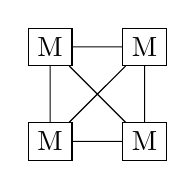
\begin{tikzpicture}[scale=1.2]
		\node[draw] (M1) at (0,0) {M};
		\node[draw] (M2) at (0,1) {M};
		\node[draw] (M3) at (1,0) {M};
		\node[draw] (M4) at (1,1) {M};
		\draw[-] (M1) -- (M2) (M1) -- (M3) (M1) -- (M4)
					(M2) -- (M3) (M2) -- (M4)
					(M3) -- (M4);
	\end{tikzpicture}
}
\subcaption{Miner node network}
\vspace{1cm}
\resizebox {0.7\columnwidth} {!} {
	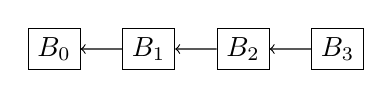
\begin{tikzpicture}	[scale=1.2]
		\node[draw] (B1) at (-1,-1) {$B_0$};
		\node[draw] (B2) at (0,-1) {$B_1$};
		\node[draw] (B3) at (1,-1) {$B_2$};
		\node[draw] (B4) at (2,-1) {$B_3$};

		\draw[->] (B4) -- (B3);
		\draw[->] (B3) -- (B2);
		\draw[->] (B2) -- (B1);
	\end{tikzpicture}
}
\subcaption{Blockchain}
\end{center}
\caption{Blockchain overview}
\label{fig:blockchain}
\end{figure}

\section{Design goals}
Before designing the system, a number of goals must be defined and an attempt made to satisfy them in the design. My design goals are listed below.

\begin{itemize}
	\item The system must be \textit{privacy preserving}. It must not be possible for a malicious user to obtain any additional information from an honest user than the information the honest user intended to release.
	\item False location proofs must be detectable. It must be possible to detect any location proofs attempting to prove false information.
	\item The system must be decentralised, and cannot rely on any central nodes. This is discussed in section \ref{ssec:centralised}.
	\item The design must conform to the desirable properties defined in OTIT (discussed in section \ref{ssec:otit}).
	\item The system must not be vulnerable to any known threats (section \ref{ssec:threats}).
\end{itemize}

\subsection{Central services} \label{ssec:centralised}
Location proof systems which rely on central noes, such as those discussed in section \ref{ssec:proof_systems}, have a fundamental weakness. These systems assume that the central node is honest, always available, and cannot be compromised by an attacker. Since the central node is in charge of coordinating the system, compromising it allows an attacker potentially unlimited control over the system. This completely violates a users privacy in a location verification system, as the central node may contain sensitive information about users and their location, or a means of retrieving sensitive information, such as decryption keys. Users of the system also have to assume that the central node is available at all times, otherwise the system is considered unavailable, or ``down''.

These problems do not occur in a decentralised location proof system, because no node is considered to be ``in charge''. This lack of authority prevents privacy breaches, but presents other issues. System coordination, which is easily maintained by the central node in a centralised system, is now maintained by each participant in the decentralised system.

\subsection{OTIT} \label{ssec:otit}
Khan et al. present the \textit{OTIT} model, a ``model for designing secure location provenance'' \cite{otit}. It defines the following 8 desirable properties of a location proof system:
\begin{itemize}
	\item[] \textbf{Chronological}: Location proofs should be ordered according to the sequence of their creation.
	\item[] \textbf{Order preserving}: The order in which the proofs were entered into the proof chain should always be maintained.
	\item[] \textbf{Verifiable}: A Verifier should be able to verify or reject the claim by the user that he has visited the given location(s).
	\item[] \textbf{Tamper evident}: A Verifier should be able to detect if the proof chain has been tampered with or modified by an unauthorised party.
	\item[] \textbf{Privacy preserved}: When the proof chain is verified for specific location proofs, privacy is preserved for the other location proofs within the chain.
	\item[] \textbf{Selective In-sequence privacy}: The user should be able to choose not to reveal some location proofs within the proof chain when seeking verification.
	\item[] \textbf{Privacy protected chronology}: The system should ensure that the user does not hide important information from the items within the subset of the proof chain.
	\item[] \textbf{Convenience and derivability}: The system shold ensure that the user does not burden the Verifier with a large amount of data to analyse in order to verify his location.
\end{itemize}

\subsection{Threats} \label{ssec:threats}
A number of related publications \cite{luo,khan} have identified various potential threats (or attacks) on location verification systems. These are outlined below.

\begin{itemize}
	\item[] \textbf{False presence}: A dishonest user tries to obtain a location proof for a false location.
	\item[] \textbf{Malicious intruders}: A malicious intruder offers to help another user prove a false location, but doesn't prove a false location for himself.
	\item[] \textbf{Curious users}: A curious user learns another user's identity while the user is acquiring the location proof.
	\item[] \textbf{Malicious applications}: The application that the user is proving his location to takes advantage of the user's information.
	\item[] \textbf{Eavesdroppers}: An eavesdropper intercepts or modifies communication between two honest users.
	\item[] \textbf{Wormhole attacks}: An attacker records network traffic in one location and replays it in another location (at another time).
	\item[] \textbf{Weak identities}: A user gives his public key or identity to another colluding user in order to create a location proof.
	\item[] \textbf{False timestamping (backdating, future dating)}: In a backdating attack, the attacker creates a location proof with a past timestamp. In future dating, the attacker creates a location proof with a future timestamp
	\item[] \textbf{Implication}: A malicious user, or group of colluding malicious users, create a false location proof for an honest user.
	\item[] \textbf{False assertion}: Two malicious users collude to create a false location proof for themselves.
	\item[] \textbf{Proof switching}: A malicious user modifies one of its existing honest proofs to spoof a false location.
	\item[] \textbf{Relay attack}: A malicious user creates a location proof with an honest user by relaying his requests through a colluding \textit{proxy user}, who is physically present at a location that the malicious user wishes to create false proofs at.
	\item[] \textbf{Sybil attack}: A Sybil attack occurs when a single malicious user of the system generates multiple \textit{pseudoidentities} and masquerades as multiple users \cite{sybil}.
\end{itemize}